\documentclass[10pt,conference,compsocconf]{IEEEtran}
\usepackage{svg}

\usepackage{hyperref}
\usepackage{graphicx}	% For figure environment


\begin{document}
\title{Nano4M - COM304}

\author{
  Sacha Godey (362191), Alexis Carreras (361573), Gabriel Taieb (360560), Adrien Bousquié (361516)\\
  \textit{COM-304 Project Proposal}
}

\maketitle

% ---------- Abstract ----------
\begin{abstract}
    We propose a specialized foundation model derived from the 4M architecture \cite{mizrahi_4m_2023}, designed specifically for handling dynamic modalities such as audio and video. Unlike the original 4M model, Nano4M addresses the inability to process temporal modalities by introducing custom-developed audio and video tokenizers. For audio, we leverage spectrogram representations inspired by MAE-AST \cite{baade_mae-ast_2022}, while for video, we employ spatio-temporal patching methods based on MaskViT \cite{gupta_maskvit_2022} and MAGVIT \cite{yu_magvit_2023}. Our approach involves training optimized tokenizers tailored explicitly for these modalities, integrating them into a unified Transformer-based architecture capable of multimodal reasoning and synchronized audio-video generation. The model will be validated against standard datasets (UCF-101, BAIR Robot Pushing, AudioSet, ESC-50), benchmarking performance against state-of-the-art methods. Ultimately, our nano4M aims to significantly enhance multimodal understanding, broaden the applicability of foundation models, and improve computational efficiency for real-world multimedia applications.
\end{abstract}


% ---------- Introduction ----------
\section{Introduction}

 The goal of our project is to develop a foundation model which is a smaller version of the 4M model \cite{mizrahi_4m_2023} specialized on dynamic elements such as video and audio. We aim to address the fact that 4M is unable to process audio and video by integrating these complex modalities, thereby enabling multimodal tasks involving synchronized audio-video generation and enhancing multimodal reasoning capabilities.

Audio and video are essential in real-world applications like content generation, accessibility tools, and multimedia communication. Incorporating these modalities into nano4M significantly increases the practical utility  of the model, making it suitable for advanced multimodal tasks such as video captioning, video-to-audio generation, and improved multimodal understanding.

% ---------- Method and Deliveries ----------
\section{Method and Deliveries}
First, we will analyze various pre-existing audio and video tokenizers and draw inspiration from them to develop our own from scratch. Our initial task will be to enhance the provided dataset in order to train our new tokenizers tailored to each format. Next, we will implement a system that enables any-to-any modality handling by incorporating the desired modalities, such as Video and Audio. Accordingly, we have the following list of extensions:

\textbf{1. Audio modality integration and tokenizer:}
We will implement an audio tokenizer based on spectrogram representations and masked audio generation inspired by MAE-AST \cite{baade_mae-ast_2022}. This includes adapting the nano4M Transformer architecture to handle spectrogram tokens and masked reconstruction.

\textbf{2. Video Modality Integration and tokenizer:}
We will also introduce video tokens using spatio-temporal patching methods inspired by MaskViT \cite{gupta_maskvit_2022} and MAGVIT \cite{yu_magvit_2023}. This involves designing a tokenizer capable of representing video sequences efficiently and adapting the Transformer architecture to model temporal dependencies.

\textbf{3. Tokenization improvements for audio and video:}
Training specialized tokenizers will be the following part, separately for audio and video to optimize reconstruction performance and alignments compared to standard off-the-shelf tokenizers.

\textbf{4. Inference strategy optimization:}
Comparing iterative decoding versus one-pass decoding methods, experimenting with sampling strategies like top-k and nucleus sampling, and evaluating trade-offs.

   
    
\begin{figure}[tbph]
  \centering
  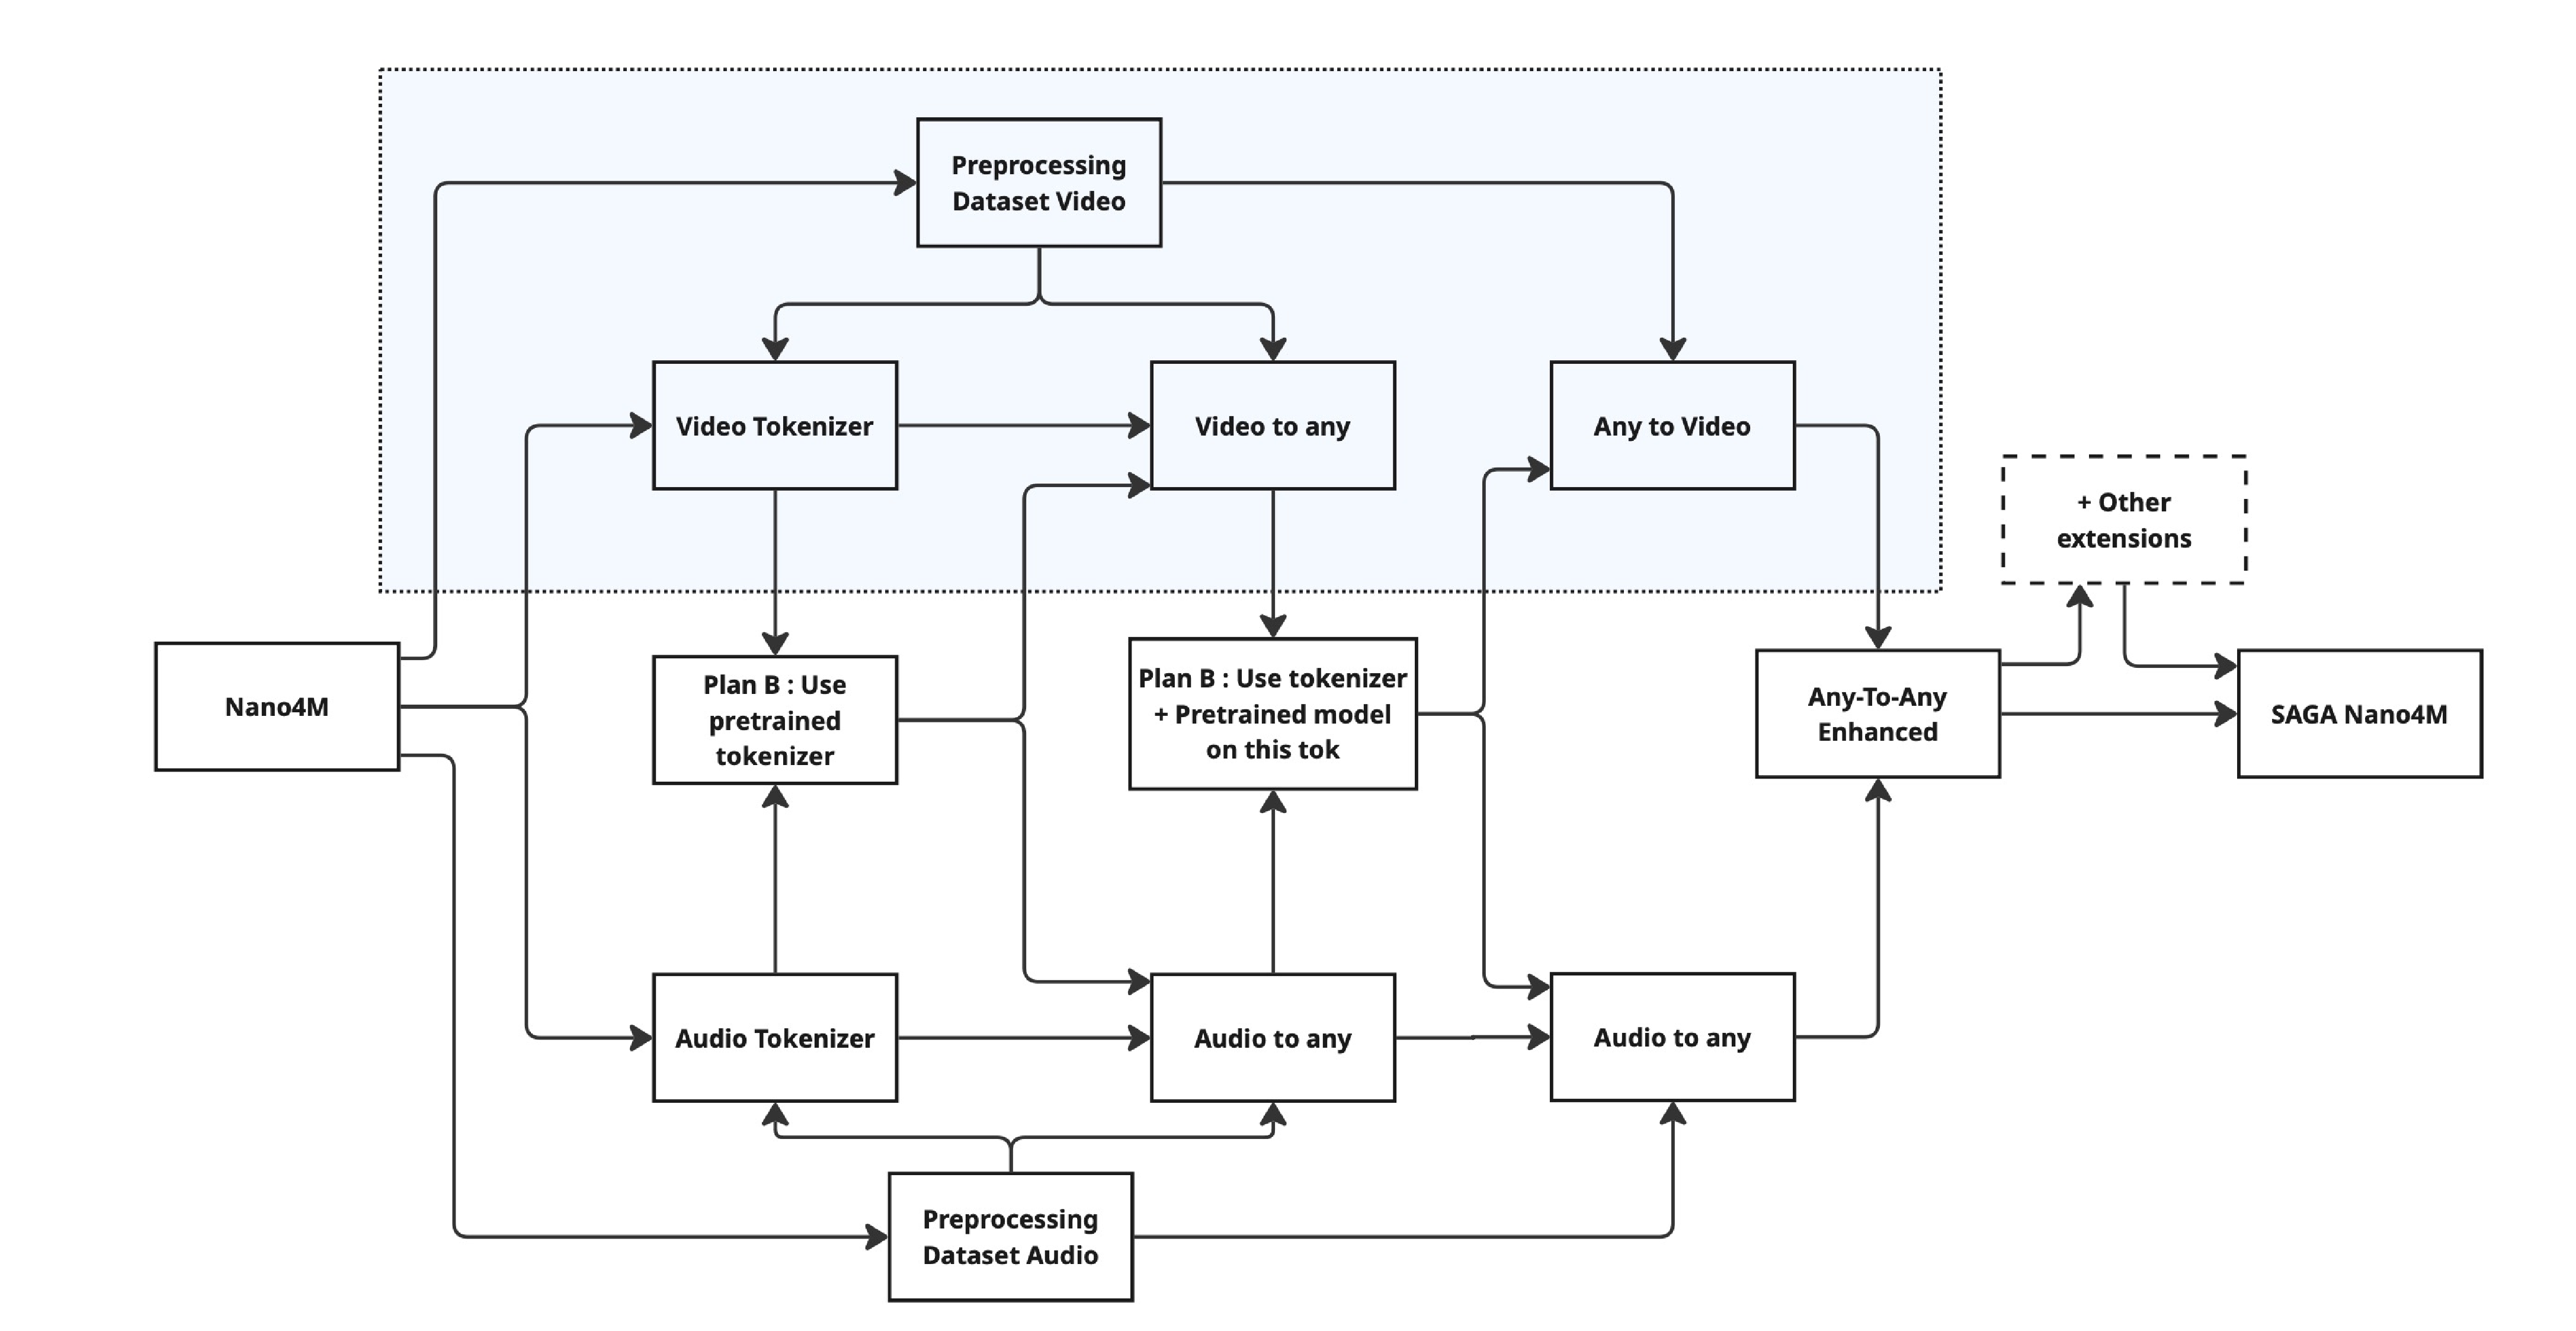
\includegraphics[width=1\columnwidth]{latex-proposal-template/Extensions.pdf}
  \caption{Overall plan of our project extensions}
  \vspace{-3mm}
  \label{fig:placeholder1}
\end{figure}

To validate our solution, we will conduct extensive benchmarking by comparing our results with state-of-the-art models using various evaluation metrics, such as mIoU as seen in the homework. Our evaluation will involve multiple test datasets with established performance benchmarks. Specifically, UCF-101 and BAIR Robot Pushing for video, and AudioSet along with ESC-50 for audio. This approach will enable us to visualize the performance of our tokenizers as well as assess the quality of the outputs generated across our newly introduced modalities.


\subsection{Expected Progress by Progress Report}
\begin{itemize}
    \item \textbf{Week 6-9:} Implement nano4M
    \item \textbf{Week 11:} Tokenizers (Video and Audio) and preprocessing of the dataset
    \item \textbf{Week 12:} Continue implementing tokenizers and implement modalities.
    \item \textbf{Week 13:} Continue modality implementation and fine tuning of the model
    \item \textbf{Week 14:} Presentation preparation.
\end{itemize}
    \textbf{Mitigation :} Due to the unknown workload associated with the tokenizer and training on a new modality, our current time allocation is an initial estimate that may be adjusted as we gain further insights into Nano4M.


% ---------- Related Work ----------
\section{Related Work}
Based on our homework experience with 4M, we observed that while 4M is robust in image generation, its temporal visualization is limited. The possible solution is to treat each video frame merely as an RGB image. In contrast, models like MAGVit \cite{yu_magvit_2023} excel in capturing temporal dynamics in videos but do not leverage the full range of image modalities offered by 4M \cite{mizrahi_4m_2023}. Our work aims to bridge this gap by developing a unified model that addresses the challenges of both approaches. Furthermore, we aim to enhance the time-dependent treatment of modalities such as audio. Audio is well tokenized by models and can be used to infer multiple other modalities\cite{tian_audiox_2025}. It would be interesting to integrate the modality treatments from these three different models into one system. This approach has already been explored by the AudioX model \cite{tian_audiox_2025}; however, our model differentiates itself by being based on 4M, offering a more comprehensive image management.


% ---------- Discussion ----------
\section{Discussion}

\subsection{Implications and Broader Impact}
Improving the 4M video tokenizer can significantly enhance usability and efficiency by reducing the current heavy processing—where tokenizing 30 frames takes about 30 seconds in the homework — thus, a 1-minute video at 24 fps would require roughly 24 minutes of tokenization. This optimization not only cuts down time and resource consumption but also lessens the computational footprint. However, incorporating a new modality and dataset increases training requirements and carbon emissions, presenting a challenging trade-off. Moreover, benchmarking with established datasets (e.g., UCF-101, BAIR Robot Pushing, AudioSet, ESC-50) will provide robust performance metrics and valuable visualizations for future multimodal projects.

\subsection{Potential Risks and Shortcomings}
Since the handling and generation of videos and audio is still a work in progress, we are aware that we will encounter some difficulties. We know that our project is ambitious and we may have to adapt the development of our model in function. Another risk could be to be limited by the computational resources because of the heavier nature of videos.
If we are not able to implement a working tokenizer, we are planning on implementing and using the MAGVIT tokenizer \cite{yu_magvit_2023}. And in case we are not able to implement the audio handling, we will focus on the video part and maybe add more modalities, e.g. frame interpolation to increase frame rate of a video.


\bibliographystyle{IEEEtran}
\bibliography{references.bib}

\end{document}

TODO: Remove this later

Extensions:
1- Lips reading (trouve un dataset)
5- Black & white to color
2- Language des signes
3- Audio description
4- Subtitles
- Multimodal reasoning & test-time compute
- Inference strategy
- Image extension (Generate a dezoomed image)
- Sound ambiance
- 

Given an input it knows the best middle modalities to generate a particular output
Have different extensions so we can 

1. What is the problem you want to solve?
2. Why is it important that this problem be solved?
3. How do you solve this problem?

Where is the template of the project proposal ?

watching 4M 21 paper citing the paper to see what they do

document yourself 4M

40 : Tokenizer
60 : Modalities
